\documentclass[11pt,a4paper]{article}

\usepackage[utf8]{inputenc}
\usepackage[margin=0.6in]{geometry}
\usepackage{amsmath}
\usepackage{booktabs}
\usepackage{enumitem}

% TikZ for visual diagrams
\usepackage{tikz}
\usetikzlibrary{arrows.meta, positioning}

\pagestyle{empty}

\begin{document}

% Header banner with Hackathon Track & National Mission context
\noindent\textbf{\large Proposal: Offline AI Agent for Intelligent Governance \& Public Services}\\[0.05cm]
\noindent{\small \textbf{Track 1:} AI for Intelligent Governance, Security \& Public Services \hfill \textbf{Innovathon 2.0} (Viksit Bharat @2047 / Mission YUVA)}\\[0.06cm]
\hrule
\vspace{0.18cm}

% =========================================================
% 1. QUICK IDEA SUMMARY
% =========================================================
\noindent\textbf{\large 1. The Idea in Short}

\vspace{0.1cm}
\noindent
Public administrative offices (Tehsils, Block Development Offices, Municipal Councils) handle thousands of citizen applications, welfare schemes, and public records every day. Administrative staff want AI to reduce clerical backlogs, but face three hard barriers:
\begin{itemize}[leftmargin=*, itemsep=1.5pt, topsep=2pt]
    \item \textbf{Data Privacy and Legal Compliance:} Citizen data (Aadhaar, land records, pension rolls) cannot be uploaded to commercial cloud AI (ChatGPT, Copilot) under the Digital Personal Data Protection (DPDP) Act 2023 and government data security directives.
    \item \textbf{Government Hardware Reality:} Most administrative computers are entry-level desktops (Core i3 or i5, 8 GB RAM, no GPU). In hilly and remote administrative blocks, internet connectivity is often slow or down.
    \item \textbf{Clerical Math and Hallucination Risk:} Public administration cannot tolerate AI errors. If an LLM hallucinates a citizen name or makes a math error in a welfare disbursement, it creates audit objections and public disputes.
\end{itemize}

\vspace{0.08cm}
\noindent
\textbf{What we are building:} An air-gapped, offline desktop AI agent with a simple graphical interface designed for government staff on budget 8 GB PCs. It automates public service workflows using a library of \textbf{Modular Governance Skills} without sending any data over the internet.

\noindent
\textbf{The core engineering trick:} The local language model (1.5B to 3B) runs entirely on the CPU and acts only as a semantic planner. It uses strict GBNF grammars to pick pre-tested Python skills. Python handles all math, name matching, and document formatting deterministically, followed by a mathematical integrity check and audit log.

\vspace{0.18cm}
\rule{\textwidth}{0.4pt}
\vspace{0.12cm}

% =========================================================
% 2. SYSTEM ARCHITECTURE DIAGRAM
% =========================================================
\noindent\textbf{\large 2. System Architecture}

\vspace{0.12cm}
\begin{figure}[h!]
\centering
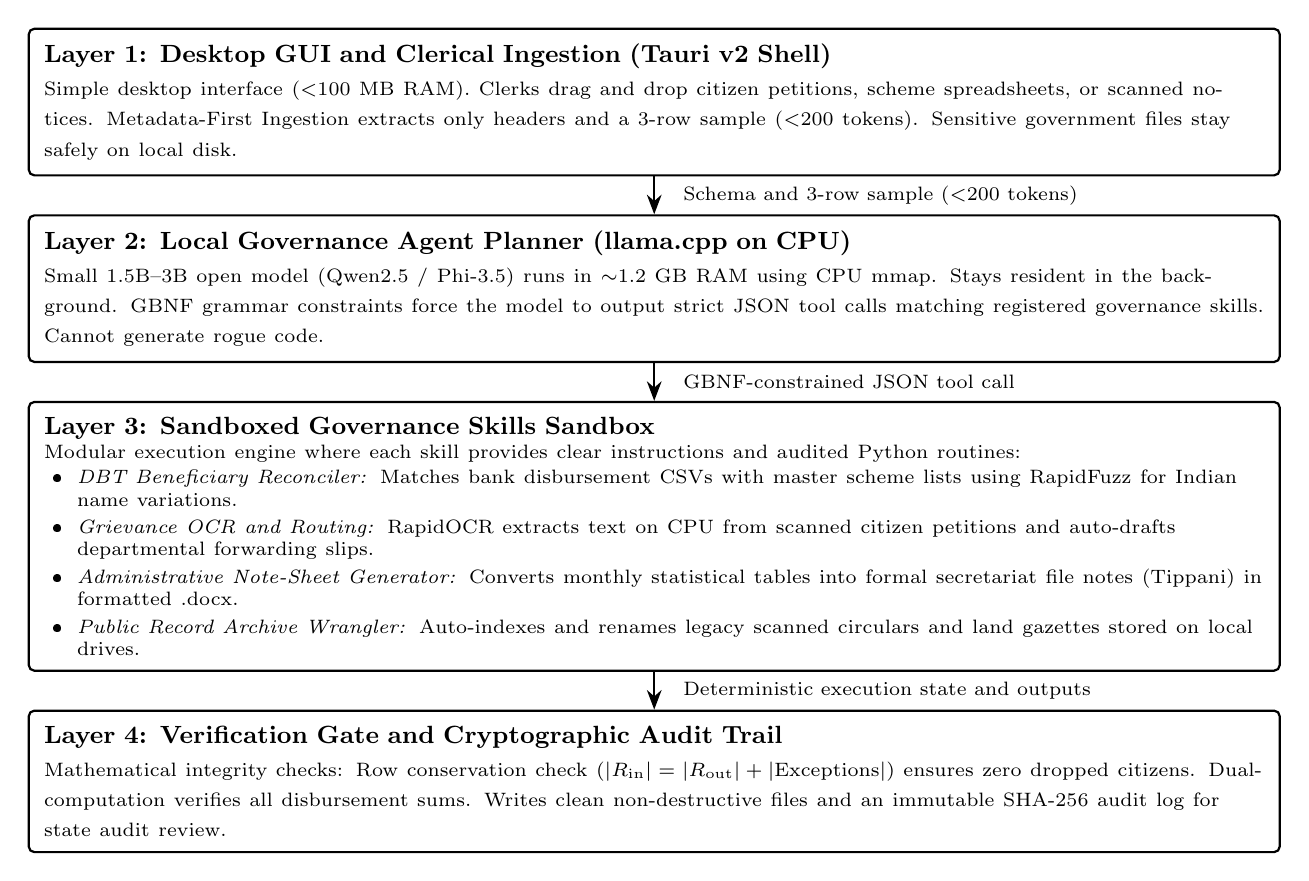
\begin{tikzpicture}[
    >=Stealth,
    font=\small,
    node distance=0.48cm,
    stage/.style={
        rectangle, draw=black, fill=white, rounded corners=2pt,
        line width=0.8pt, align=left, inner sep=5.5pt,
        text width=15.5cm, minimum height=0.9cm
    },
    arrow/.style={->, line width=0.9pt, draw=black},
    flowlabel/.style={font=\scriptsize, fill=white, inner sep=1.5pt}
]

\node[stage] (s1) {
    \textbf{Layer 1: Desktop GUI and Clerical Ingestion (Tauri v2 Shell)}\\[0.03cm]
    \scriptsize Simple desktop interface ($<$100 MB RAM). Clerks drag and drop citizen petitions, scheme spreadsheets, or scanned notices.
    Metadata-First Ingestion extracts only headers and a 3-row sample ($<$200 tokens). Sensitive government files stay safely on local disk.
};

\node[stage, below=of s1] (s2) {
    \textbf{Layer 2: Local Governance Agent Planner (llama.cpp on CPU)}\\[0.03cm]
    \scriptsize Small 1.5B--3B open model (Qwen2.5 / Phi-3.5) runs in $\sim$1.2 GB RAM using CPU mmap. Stays resident in the background.
    GBNF grammar constraints force the model to output strict JSON tool calls matching registered governance skills. Cannot generate rogue code.
};

\node[stage, below=of s2] (s3) {
    \textbf{Layer 3: Sandboxed Governance Skills Sandbox}\\[0.03cm]
    \scriptsize Modular execution engine where each skill provides clear instructions and audited Python routines:
    \begin{itemize}[leftmargin=1.5em, itemsep=0pt, topsep=1pt]
        \item \textit{DBT Beneficiary Reconciler:} Matches bank disbursement CSVs with master scheme lists using RapidFuzz for Indian name variations.
        \item \textit{Grievance OCR and Routing:} RapidOCR extracts text on CPU from scanned citizen petitions and auto-drafts departmental forwarding slips.
        \item \textit{Administrative Note-Sheet Generator:} Converts monthly statistical tables into formal secretariat file notes (Tippani) in formatted .docx.
        \item \textit{Public Record Archive Wrangler:} Auto-indexes and renames legacy scanned circulars and land gazettes stored on local drives.
    \end{itemize}
};

\node[stage, below=of s3] (s4) {
    \textbf{Layer 4: Verification Gate and Cryptographic Audit Trail}\\[0.03cm]
    \scriptsize Mathematical integrity checks: Row conservation check ($|R_{\text{in}}| = |R_{\text{out}}| + |\text{Exceptions}|$) ensures zero dropped citizens.
    Dual-computation verifies all disbursement sums. Writes clean non-destructive files and an immutable SHA-256 audit log for state audit review.
};

% Labeled Arrows
\draw[arrow] (s1) -- node[flowlabel, right=0.3cm] {Schema and 3-row sample ($<$200 tokens)} (s2);
\draw[arrow] (s2) -- node[flowlabel, right=0.3cm] {GBNF-constrained JSON tool call} (s3);
\draw[arrow] (s3) -- node[flowlabel, right=0.3cm] {Deterministic execution state and outputs} (s4);

\end{tikzpicture}
\end{figure}

\vspace{-0.25cm}
\rule{\textwidth}{0.4pt}

\newpage

% =========================================================
% 3. WHY THIS ARCHITECTURE WORKS
% =========================================================
\noindent\textbf{\large 3. Why This Architecture Works for Public Administration}

\vspace{0.15cm}
\noindent
Comparison with existing commercial and open-source tools in government settings:

\vspace{0.2cm}

\renewcommand{\arraystretch}{1.3}
\small

\noindent
\begin{tabular}{|p{2.8cm}|p{4.2cm}|p{4.2cm}|p{4.2cm}|}
\hline
\textbf{Governance Need} & \textbf{Commercial Cloud AI (Copilot / ChatGPT)} & \textbf{Developer CLI Agents (Claude Code / OpenDevin)} & \textbf{Our Offline Governance Agent} \\
\hline

\textbf{Data Security and Air-Gapping}
& Violates DPDP Act 2023. Sends citizen PII and land records to foreign cloud servers.
& Sends data to paid cloud model APIs; cannot operate inside closed government LAN.
& \textbf{100\% Air-Gapped.} Runs entirely on local PC disk. Zero telemetry and zero data leaks.
\\
\hline

\textbf{Clerical Usability}
& Chat interface only. Gives raw conversational text; does not format formal office orders.
& Terminal command-line only. Requires developer and coding knowledge.
& \textbf{Desktop GUI for Clerks.} Drag-and-drop files, live visual diff preview, and one-click export.
\\
\hline

\textbf{Accuracy and Auditability}
& Hallucinates numbers and guesses totals. No legal audit trail for state vigilance.
& Tries to write unvetted scripts on the fly, leading to runtime and syntax crashes.
& \textbf{Zero Hallucinations.} GBNF grammar rails + deterministic Python + SHA-256 audit log.
\\
\hline

\textbf{Government Hardware Fit}
& Needs continuous high-speed broadband and costly monthly subscriptions.
& Requires high-end developer workstations with dedicated GPUs and 16 GB+ RAM.
& \textbf{Runs on GeM Budget Desktops.} Core i3 / 8 GB RAM with $>$1.7 GB free memory headroom.
\\
\hline

\textbf{Local Offline OCR}
& Requires uploading document images to cloud vision APIs.
& No built-in lightweight local document OCR engine.
& \textbf{CPU RapidOCR.} Reads paper petitions and receipts on local machine without internet.
\\
\hline

\end{tabular}

\vspace{0.4cm}

% =========================================================
% 4. HARDWARE NUMBERS & DEMO SKILLS
% =========================================================
\noindent\textbf{\large 4. Hardware Budget and Planned Live Demonstration}

\vspace{0.2cm}
\noindent
\begin{minipage}[t]{0.45\textwidth}
\textbf{Memory Budget (Standard 8 GB Govt PC):}\\[0.15cm]
\small
\begin{tabular}{p{4.2cm} r}
\toprule
\textbf{Component} & \textbf{RAM} \\
\midrule
Windows + Antivirus + Browser & 4.5 GB \\
Model Weights (1.5B--3B Q4) & 1.2 GB \\
KV Context Buffer (2048 tokens) & 0.2 GB \\
Tauri Desktop UI & 0.1 GB \\
Python Sandbox Worker & 0.3 GB \\
\midrule
\textbf{Total System Used} & \textbf{6.3 GB} \\
\textbf{Remaining Free Buffer} & \textbf{$>$1.7 GB} \\
\bottomrule
\end{tabular}
\end{minipage}
\hfill
\begin{minipage}[t]{0.50\textwidth}
\textbf{Live Demo Scenarios (Innovathon 2.0):}\\[0.15cm]
\small
\begin{itemize}[leftmargin=1.2em, itemsep=3.5pt]
    \item \textbf{DBT Scheme Reconciler:}\\ Matches 500 beneficiary records against bank transfer CSVs using RapidFuzz, isolates unpaid cases, and writes native Excel totals.
    \item \textbf{Citizen Grievance OCR:}\\ Scans a paper petition regarding local water supply using CPU OCR, classifies urgency, and auto-drafts a forwarding note.
    \item \textbf{Administrative Note-Sheet:}\\ Converts monthly block progress tables into a formal secretariat note-sheet (.docx) with official styling.
    \item \textbf{Cryptographic Audit Trail:}\\ Exports a tamper-evident SHA-256 JSON audit log confirming zero dropped citizen records.
\end{itemize}
\end{minipage}

\vspace{0.4cm}
\begin{center}
\small
\textbf{Execution Time:} 15 to 25 seconds \quad $\bullet$ \quad
\textbf{Target Hardware:} 8 GB RAM laptop (No GPU) \quad $\bullet$ \quad
\textbf{Deployment:} 100\% Air-Gapped / Offline
\end{center}

\end{document}
